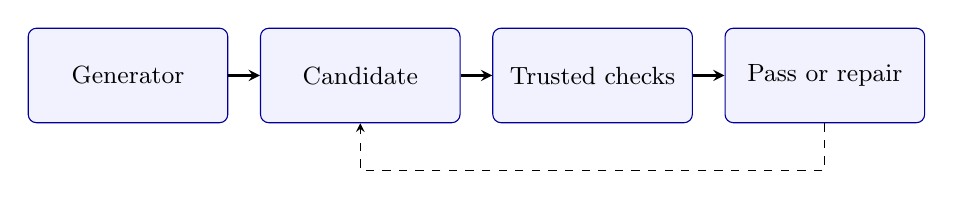
\begin{tikzpicture}[nodebox/.style={draw=blue!60!black,fill=blue!5,rounded corners=3pt,minimum height=12mm,text width=23mm,align=center,font=\small},>=stealth]
\node[nodebox] (n0) at (0.00,0.00) {Generator};
\node[nodebox] (n1) at (2.95,0.00) {Candidate};
\node[nodebox] (n2) at (5.90,0.00) {Trusted checks};
\node[nodebox] (n3) at (8.85,0.00) {Pass or repair};
\draw[->,thick] (n0.east) -- (n1.west);
\draw[->,thick] (n1.east) -- (n2.west);
\draw[->,thick] (n2.east) -- (n3.west);
\draw[->,dashed] (n3.south) -- ++(0,-.6) -| (n1.south);
\end{tikzpicture}
